\documentclass[aspectratio=169,12pt]{beamer}
\usepackage[utf8]{inputenc}
\usepackage{amsmath, amssymb}
\usepackage{booktabs}
\usepackage{colortbl}
\usepackage{hyperref}
\usepackage{makecell}
\usepackage{ragged2e}
\usepackage{bytefield}
\usepackage{tikz}
\usetikzlibrary{arrows.meta, positioning, shapes.geometric, calc, tikzmark, shapes.misc}
\usetheme{Madrid}

% Define custom ALU shape command
\newcommand{\drawAdder}[1]{
    \node[inner sep=0] (adder) at #1 {
        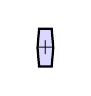
\begin{tikzpicture}[scale=0.4]
            \coordinate (tl) at (-0.2, 0.6);
            \coordinate (tr) at (0.2, 0.6);
            \coordinate (ml) at (-0.25, 0);
            \coordinate (mr) at (0.25, 0);
            \coordinate (bl) at (-0.2, -0.6);
            \coordinate (br) at (0.2, -0.6);
            
            \fill[blue!15] (tl) -- (tr) -- (mr) -- (br) -- (bl) -- (ml) -- cycle;
            \draw[thick] (tl) -- (tr) -- (mr) -- (br) -- (bl) -- (ml) -- cycle;
            
            \node[font=\scriptsize] at (0, 0) {+};
        \end{tikzpicture}
    };
}

% Define macro for placing adders in pipeline with configurable location and optional rotation
% Usage: \placeAdder{prefix}{x,y}[rotation angle]
\newcommand{\placeAdder}[3][0]{%
    \begin{scope}[shift={(#2)}, scale=0.8, rotate=#1]
        \coordinate (#3_adder) at (0,0);
        % Trapezoid coordinates
        \coordinate (toptopleft) at (0, 0.4);
        \coordinate (topbottomleft) at (0, 0.15);
        \coordinate (left) at (0.1, 0);
        \coordinate (bottomtopleft) at (0, -0.15);
        \coordinate (bottombottomleft) at (0, -0.4);
        \coordinate (topright) at (0.3, 0.2);
        \coordinate (bottomright) at (0.3, -0.2);
        
        % Draw the trapezoid
        \fill[blue!15] (toptopleft) -- (topbottomleft) -- (left) -- (bottomtopleft) -- (bottombottomleft) -- (bottomright) -- (topright) -- cycle;
        \draw[thick] (toptopleft) -- (topbottomleft) -- (left) -- (bottomtopleft) -- (bottombottomleft) -- (bottomright) -- (topright) -- cycle;
        
        % Add + text
        \node at (0.16, 0) {\tiny +};

        \coordinate (#3_adder_input1) at (0, 0.3);
        \coordinate (#3_adder_input2) at (0, -0.3);
        \coordinate (#3_adder_output) at (0.3, 0);
    \end{scope}
}

% Define macro for pipeline diagram
% Usage: \drawPipelineDiagram[x,y] - optional position, defaults to (0,0)
\newcommand{\drawPipelineDiagram}[1][0,0]{%
    \scalebox{0.85}{%
    \begin{tikzpicture}[shift={(#1)},
        component/.style={draw, thick, minimum height=0.8cm},
        latch/.style={draw, thick, fill=yellow!20, minimum width=0.2cm, minimum height=4cm},
        stage/.style={font=\bfseries},
        label/.style={font=\tiny},
        port/.style={font=\tiny, inner sep=0.035cm}
    ]
        % Define origin node for relative positioning
        \coordinate (origin) at (0,0);
        
        % Pipeline latches - positioned relative to origin
        \node[latch] (L1) at ([shift={(3,2)}]origin) {};
        \node[latch] (L2) at ([shift={(3,0)}]L1) {};
        \node[latch] (L3) at ([shift={(3.5,0)}]L2) {};
        \node[latch] (L4) at ([shift={(2.5,0)}]L3) {};
        
        % Stage labels - positioned relative to latches
        \node[stage] at ([yshift=4cm]origin |- L1.north) {Fetch};
        \node[stage] at ([yshift=4cm]L1.north) {Decode};
        \node[stage] at ([yshift=4cm, xshift=1cm]L2.north) {Execute};
        \node[stage] at ([yshift=4cm, xshift=0.5cm]L3.north) {Memory};
        \node[stage] at ([yshift=4cm, xshift=0.5cm]L4.north) {WB};
        
        % Fetch Stage
        % PC MUX (rotate=90: output on west) - positioned relative to PC
        \placeMux[90]{$(origin) + (0.3,4.5)$}{pc}{blue!20}

        % PC - positioned relative to L1
        \node[component, fill=blue!20, minimum width=0.6cm, minimum height=0.6cm] (PC) at ([xshift=-2.5cm, yshift=0]L1.center) {\small PC};

        % ICache - positioned relative to L1
        \node[component, fill=purple!20, minimum width=1.2cm, minimum height=2cm] (ICache) at ([xshift=-1cm, yshift=0]L1.center) {};
        \node[align=center] at ([yshift=0.6cm]ICache.center) {\footnotesize inst.\\[-0.14cm]\footnotesize cache};
 
        % PC adder - positioned relative to PC
        \placeAdder{$(PC.center) + (0.7,1.8)$}{fe}
        \node[left, font=\tiny] (four) at ([xshift=-0.3cm]fe_adder_input1) {4};
        
        % Decode Stage - positioned between L1 and L2, with vertical offset
        \node[component, fill=pink!30, minimum width=1.2cm, minimum height=1.8cm] (RF) at ($(L1.east)!0.5!(L2.west) + (0,0.41)$) {};
        \node[align=center] at ([yshift=-0.35cm]RF.north) {\footnotesize register\\[-0.11cm]\footnotesize file};
        
        % Register file input ports (left side, inside the box)
        \node[port] (rf_src1) at ([xshift=-0.4cm, yshift=0.1cm]RF.center) {~src1};
        \node[port] (rf_src2) at ([xshift=-0.4cm, yshift=-0.3cm]RF.center) {~src2};
        \node[port] (rf_dst) at ([xshift=-0.35cm, yshift=-0.7cm]RF.center) {dst};
        
        % Register file selector coordinate (slightly left of dst)
        \coordinate (rf_selector) at ([xshift=-0.1cm]rf_dst.south);
        
        % Register file output ports (right side, aligned to right edge)
        \node[port, anchor=east] (rf_src1_data) at ([xshift=0.6cm, yshift=0.07cm]RF.center) {src1};
        \node[port, anchor=east] (rf_data1) at ([yshift=-0.15cm]rf_src1_data.east) {data};
        \node[port, anchor=east] (rf_src2_data) at ([xshift=0.6cm, yshift=-0.37cm]RF.center) {src2};
        \node[port, anchor=east] (rf_data2) at ([yshift=-0.15cm]rf_src2_data.east) {data};
        
        % Sign extension - positioned relative to register file  
        \node[component, fill=green!20, ellipse, minimum width=0.4cm, minimum height=0.3cm, align=center] (SignExt) at ([xshift=0.6cm, yshift=-1.5cm]RF.center) {
            \scriptsize sign\\[-0.25cm]\scriptsize ext.
        };
        
        % Execute Stage
        % Execute adder - positioned relative to L2
        \placeAdder{$(L2.east)!0.5!(L3.west) + (0,1.56)$}{ex}
        
        % Execute stage ALU source MUX (rotate=270: output on north, inputs on south) - relative to L2/L3
        \placeMux[270]{$(L2.east)!0.5!(L3.west) + (0,-0.32)$}{exe}{green!20}
        
        % ALU - positioned between L2 and L3, aligned with register file outputs
        \begin{scope}[shift={($(L2.east)!0.65!(L3.west) + (0,0)$)}, scale=0.8]
            \coordinate (ALU) at (0,0);
            % Trapezoid coordinates
            \coordinate (toptopleft) at (0, 0.8);
            \coordinate (topbottomleft) at (0, 0.3);
            \coordinate (left) at (0.2, 0);
            \coordinate (bottomtopleft) at (0, -0.3);
            \coordinate (bottombottomleft) at (0, -0.8);
            \coordinate (topright) at (0.6, 0.4);
            \coordinate (bottomright) at (0.6, -0.4);
            
            % Draw the trapezoid
            \fill[green!15] (toptopleft) -- (topbottomleft) -- (left) -- (bottomtopleft) -- (bottombottomleft) -- (bottomright) -- (topright) -- cycle;
            \draw[thick] (toptopleft) -- (topbottomleft) -- (left) -- (bottomtopleft) -- (bottombottomleft) -- (bottomright) -- (topright) -- cycle;
            
            % Add ALU text (rotated and smaller)
            \node[rotate=90, font=\tiny] at (0.31, 0) {ALU};

            \coordinate (alu_input1) at (0, 0.4);
            \coordinate (alu_input2) at (0, -0.4);
            \coordinate (alu_output) at (0.6, 0);
        \end{scope}
        
        % Memory Stage - positioned relative to L4
        \node[component, fill=brown!20, minimum width=1.2cm, minimum height=2cm] (DCache) at ([xshift=-1.2cm, yshift=0]L4.center) {};
        \node[align=center] at ([yshift=0.6cm]DCache.center) {\footnotesize data\\[-0.14cm]\footnotesize cache};

        % Data Cache ports (aligned to left side of box)
        \node[port, anchor=west] (dc_addr) at ([xshift=-0.62cm, yshift=0cm]DCache.center) {address};
        \node[port, anchor=west] (dc_data) at ([xshift=-0.62cm, yshift=-0.7cm]DCache.center) {data};

        % DCache output port
        \node[port, anchor=east] (dc_data_out) at ([xshift=0.65cm, yshift=0cm]DCache.center){};
        
        % Write Back Stage MUX (rotate=-90: output on east, inputs on north/south) - relative to L4
        \placeMux[270]{$(L4.east) + (0.8,-0.21)$}{wb}{green!20}
        
        % Main data path connections
        \draw[blue, thick, ->] (four) -- (fe_adder_input1);
        \draw[blue, thick, ->] (pcmux_out) -- ++(-0.4,0) |- (PC.west);
        \draw[blue, thick, ->] (PC.east) -- (ICache);
        \draw[blue, thick, ->] (PC.east) -- ++(0.1,0) |- (fe_adder_input2);
        \draw[->] (ICache) -- (L1);

        \draw[blue, thick, ->] (fe_adder_output) -- (fe_adder_output -| L1.west);
        \draw[blue, thick, ->] (fe_adder_output) -- ++(0.3,0) |- (pcmux_in1);
        \draw[blue, thick, ->] (fe_adder_output -| L1.east) -- (fe_adder_output -| L2.west);
        \draw[blue, thick, ->] (fe_adder_output -| L2.east) -- ++(0.3,0) |- (ex_adder_input1);
        
        % From L1 to Register File inputs
        \draw[->] (L1.east) -- ++(0.3,0) |- (rf_src1.west);
        \draw[->] (L1.east) -- ++(0.3,0) |- (rf_src2.west);
        \draw[->] (L1.east) -- ++(0.3,0) |- (SignExt.west);

        \draw[->] (L1.east) -- ++(0.3,0) |- ([yshift=-0.8cm]SignExt -| L2.west);
        \draw[->] ([yshift=-0.8cm]SignExt -| L2.east) -- ([yshift=-0.8cm]SignExt -| L3.west);
        \draw[->] ([yshift=-0.8cm]SignExt -| L3.east) -- ([yshift=-0.8cm]SignExt -| L4.west);
        \draw[->] ([yshift=-0.8cm]SignExt -| L4.east) -- ++(0.3, 0) -- ++(0, -0.2) -| (rf_dst.south);

        % From L1 for "instruction" title
        \draw[->] (ICache -| L1.east) -- ++(0.3,0) node[yshift=0.55cm,rotate=90,above] {\tiny{}instruction}; 

        % From Register File outputs to L2
        \draw[green, thick, ->] ([yshift=-0.01cm]rf_data1.east) -- ([yshift=-0.01cm]rf_data1.east -| L2.west);
        \draw[green, thick, ->] (rf_data2.east) -- (rf_data2.east -| L2.west);
        \draw[green, thick, ->] (SignExt.east) -- (SignExt.east -| L2.west);
        
        % From L2 to Execute components
        \draw[green, thick, ->] ([yshift=-0.01cm]rf_data1.east -| L2.east) -- ++(0.2,0) |- (alu_input1);
        \draw[green, thick, ->] (rf_data2.east -| L2.east) -- (exemux_in1);
        \draw[green, thick, ->] (SignExt.east -| L2.east) -- ++(0.3,0) |- (exemux_in2);
        \draw[green, thick, ->] (SignExt.east -| L2.east) -- ++(0.3,0) |- (ex_adder_input2);
        
        % MUX to ALU
        \draw[green, thick, ->] (exemux_out) -- ++(0.3,0) |- (alu_input2);
        
        % ALU and adder to L3
        \draw[green, thick, ->] (alu_output) -- (L3.west |- alu_output);
        \draw[blue, thick, ->] (ex_adder_output) -- (L3.west |- ex_adder_output);
        \draw[blue, thick, ->] (L3.east |- ex_adder_output) -- ++(0.25,0) |- (pcmux_in2);
        
        % L3 to Memory and from
        \draw[green, thick, ->] (alu_output -| L3.east) -- (dc_addr.west);
        \draw[green, thick, ->] (dc_data.east -| L3.east) -- (dc_data.west);
        \draw[green, thick, ->] (dc_data.east -| L3.east) -- ++(0.3,0) |- ([yshift=-1.3cm]L4.west);
        \draw[green, thick, ->] (dc_data_out) -- (dc_data_out -| L4.west);
        
        % L4 to WB mux - ALU result and memory data
        \draw[green, thick, ->] (alu_output -| L4.east) -- (wbmux_in1);
        \draw[green, thick, ->] ([yshift=-1.3cm]L4.east) -- ++(0.3,0) |- (wbmux_in2);
        
        % Write back path from mux output
        \draw[green, thick, ->] (wbmux_out) -- ++(0.3,0) -- ++(0,-2.2) -| (rf_selector);
        
        % PC MUX inputs: branch target from L3, branch from L2, and PC+4
        \draw[orange!70, thick, ->] (alu_output -| L3.east) -- ++(0.35,0) -- ++(0,3.3) -| (pcmux_selectorup);
        
        % Code on the left (temporary - should be moved outside for flexibility)
        \node[anchor=east, font=\footnotesize\ttfamily] at (-1.5,1.5) {
            \begin{tabular}{rl}
                0 & or\\
                4 & jcc 50H\\
                8 & and\\
                12 & sw\\
                16 & sub
            \end{tabular}
        };
        
    \end{tikzpicture}
    }%
}

% Define macro for placing MUX with configurable location, rotation, and fill color
% Usage: \placeMux[rotation]{x,y}{prefix}{fill color}
% rotation: angle in degrees (default 0)
% x,y: position
% prefix: name prefix for coordinates
% fill color: color for the mux (e.g., blue!20)
\newcommand{\placeMux}[4][0]{%
    \node[trapezium, trapezium left angle=70, trapezium right angle=70,
          trapezium stretches=true, minimum height=0.3cm, minimum width=1cm,
          draw, thick, fill=#4, rotate=#1] (#3mux) at (#2) {};
    
    % Define input/output coordinates based on rotation only
    % For trapezoid: unrotated has narrow left, wide right
    % Inputs should be on the wide side, output on narrow side
    \ifnum#1=90
        % Rotation 90: narrow side moves to bottom, wide side to top
        % So output should be on south (narrow), inputs on north (wide)
        \coordinate (#3mux_in1) at ([yshift=-0.2cm]#3mux.south);
        \coordinate (#3mux_in2) at ([yshift=0.2cm]#3mux.south);
        \coordinate (#3mux_out) at (#3mux.north);
        % Selector positions
        \coordinate (#3mux_selectorup) at (#3mux.east);
        \coordinate (#3mux_selectordown) at (#3mux.west);
    \else\ifnum#1=180
        % Rotation 180: narrow side moves to right, wide side to left
        % So output on east (narrow), inputs on west (wide)
        \coordinate (#3mux_in1) at ([yshift=0.2cm]#3mux.west);
        \coordinate (#3mux_in2) at ([yshift=-0.2cm]#3mux.west);
        \coordinate (#3mux_out) at (#3mux.east);
        % Selector positions
        \coordinate (#3mux_selectorup) at (#3mux.south);
        \coordinate (#3mux_selectordown) at (#3mux.north);
   \else\ifnum#1=270
        % Rotation 270: narrow side moves to top, wide side to bottom
        % So output on north (narrow), inputs on south (wide)
        \coordinate (#3mux_in1) at ([yshift=0.2cm]#3mux.south);
        \coordinate (#3mux_in2) at ([yshift=-0.2cm]#3mux.south);
        \coordinate (#3mux_out) at (#3mux.north);
        % Selector positions
        \coordinate (#3mux_selectorup) at (#3mux.west);
        \coordinate (#3mux_selectordown) at (#3mux.east);
    \else
        % Default (0 degrees): narrow left, wide right
        % Output on west (narrow), inputs on east (wide)
        \coordinate (#3mux_in1) at ([yshift=0.2cm]#3mux.east);
        \coordinate (#3mux_in2) at ([yshift=-0.2cm]#3mux.east);
        \coordinate (#3mux_out) at (#3mux.west);
        % Selector positions
        \coordinate (#3mux_selectorup) at (#3mux.north);
        \coordinate (#3mux_selectordown) at (#3mux.south);
    \fi\fi\fi
}

\title{Computer Structure}
\subtitle{Pipeline}
\author{Lihu Rappoport}
\date{}

\begin{document}

\frame{\titlepage}




%% Slide: A Basic Processor
\begin{frame}{A Basic Processor}
    \centering
    \begin{tikzpicture}[scale=0.8]
        % Placeholder for processor diagram
        \node[draw, rectangle, minimum width=12cm, minimum height=6cm, dashed, align=center] {
            \Large Processor Pipeline Diagram\\
            \normalsize (Fetch $\rightarrow$ Decode $\rightarrow$ Execute $\rightarrow$ Memory $\rightarrow$ Write Back)
        };
    \end{tikzpicture}
\end{frame}

%% Slide: Pipelined Car Assembly
\begin{frame}{Pipelining Instructions}
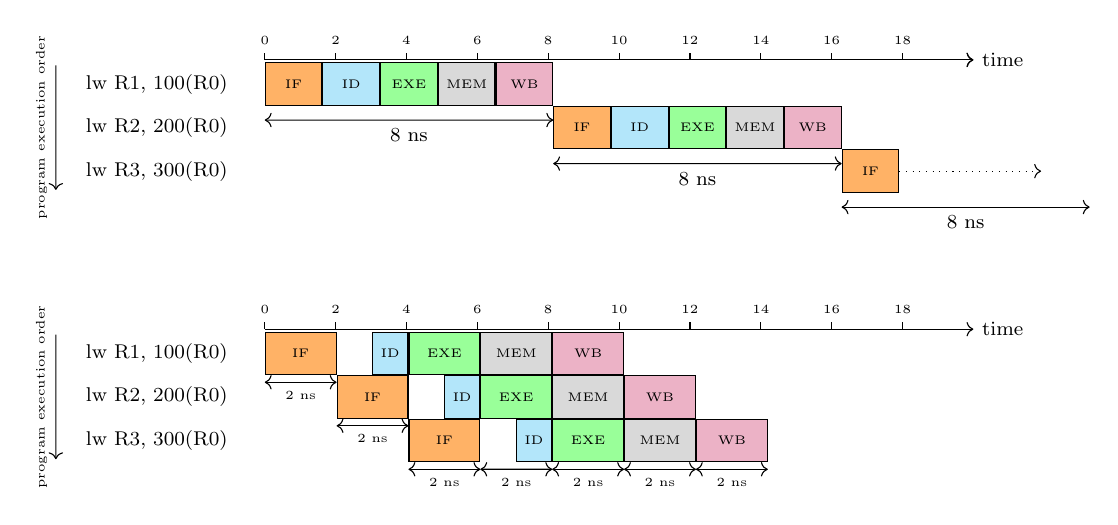
\begin{tikzpicture}[scale=0.9, transform shape,
    stage/.style={draw, minimum height=6mm, minimum width=8mm, font=\tiny, align=center, inner sep=1pt},
    fetch/.style={stage, fill=orange!60},
    reg/.style={stage, fill=cyan!30},
    alu/.style={stage, fill=green!40},
    mem/.style={stage, fill=gray!30},
    wb/.style={stage, fill=purple!30},
    pfetch/.style={stage, fill=orange!60, minimum width=10mm},
    preg/.style={stage, fill=cyan!30, minimum width=5mm},
    palu/.style={stage, fill=green!40, minimum width=10mm},
    pmem/.style={stage, fill=gray!30, minimum width=10mm},
    pwb/.style={stage, fill=purple!30, minimum width=10mm},]


% First pipeline diagram (non-pipelined)

% Time axis for first diagram with ticks above
\coordinate (timeline_start) at (1, 1.5);
\coordinate (timeline_end) at (11, 1.5);
\draw[->] (timeline_start) -- (timeline_end);
\draw[->] (timeline_start) -- (timeline_end)
  node[pos=1, right]{\footnotesize time};

\foreach \x/\t in {1/0, 2/2, 3/4, 4/6, 5/8, 6/10, 7/12, 8/14, 9/16, 10/18} {
    \draw (\x, 1.5) -- (\x, 1.6);  % tick marks
    \node[above] (t1-\t) at (\x, 1.6) {\tiny \t};
}

% First instruction row
\node[fetch, anchor=north west] (f1) at ([yshift=-1]timeline_start) {IF};
\node[anchor=east] (f1ins) at ([xshift=-4mm]f1.west) {\footnotesize lw R1, 100(R0)};
\node[reg, anchor=west] (r1a) at (f1.east) {ID};
\node[alu, anchor=west] (a1) at (r1a.east) {EXE};
\node[mem, anchor=west] (m1) at (a1.east) {MEM};
\node[wb, anchor=west] (r1b) at (m1.east) {WB};

% Second instruction row  
\node[fetch, anchor=north west] (f2) at (r1b.south east) {IF};
\node (f2ins) at (f1ins |- f2) {\footnotesize lw R2, 200(R0)};
\node[reg, anchor=west] (r2a) at (f2.east) {ID};
\node[alu, anchor=west] (a2) at (r2a.east) {EXE};
\node[mem, anchor=west] (m2) at (a2.east) {MEM};
\node[wb, anchor=west] (r2b) at (m2.east) {WB};

% Third instruction row
\node[fetch, anchor=north west] (f3) at (r2b.south east) {IF};
\node (f3ins) at (f1ins |- f3) {\footnotesize lw R3, 300(R0)};
\draw[dotted, ->] (f3.east) -- ++(2, 0);

% Timing annotations using relative positioning
\draw[<->] ([yshift=-2mm]f1.south west) -- node[below] {\footnotesize 8 ns} ([yshift=-2mm]r1b.south east);

\draw[<->] ([yshift=-2mm]f2.south west) -- node[below] {\footnotesize 8 ns} ([yshift=-2mm]r2b.south east);

\draw[<->] ([yshift=-2mm]f3.south west) -- node[below] {\footnotesize 8 ns} ++(3.5, 0);

% Vertical arrow for execution order - relative to instructions
\draw[->] 
  ([xshift=-3mm]f1ins.north west)
    -- node[rotate=90, anchor=south]{\tiny program execution order}
  ([xshift=-3mm]f3ins.south west);


% Second pipeline diagram (pipelined) - moved higher

% Time axis for second diagram
\coordinate (ptimeline_start) at (1, -2.3);
\coordinate (ptimeline_end) at (11, -2.3);

\draw[->] (ptimeline_start) -- (ptimeline_end)
  node[pos=1, right]{\footnotesize time};
\foreach \x/\t in {1/0, 2/2, 3/4, 4/6, 5/8, 6/10, 7/12, 8/14, 9/16, 10/18} {
    \draw (\x, -2.3) -- (\x, -2.2);  % tick marks
    \node[above] (t2-\t) at (\x, -2.2) {\tiny \t};
}

% First instruction (pipelined)
\node[pfetch, anchor=north west] (pf1) at ([yshift=-1]ptimeline_start) {IF};
\node[anchor=east] (pf1ins) at ([xshift=-4mm]pf1.west) {\footnotesize lw R1, 100(R0)};
\node[preg, anchor=west] (pr1a) at ([xshift=5mm]pf1.east) {ID};
\node[palu, anchor=west] (pa1) at (pr1a.east) {EXE};
\node[pmem, anchor=west] (pm1) at (pa1.east) {MEM};
\node[pwb, anchor=west] (pr1b) at (pm1.east) {WB};

% Second instruction (pipelined - starts after first Inst Fetch)
\node[pfetch, anchor=north west] (pf2) at (pf1.south east) {IF};
\node (pf2ins) at (pf1ins |- pf2) {\footnotesize lw R2, 200(R0)};
\node[preg, anchor=west] (pr2a) at ([xshift=5mm]pf2.east) {ID};
\node[palu, anchor=west] (pa2) at (pr2a.east) {EXE};
\node[pmem, anchor=west] (pm2) at (pa2.east) {MEM};
\node[pwb, anchor=west] (pr2b) at (pm2.east) {WB};

% Third instruction (pipelined - starts after second Inst Fetch)
\node[pfetch, anchor=north west] (pf3) at (pf2.south east) {IF};
\node (pf3ins) at (pf1ins |- pf3) {\footnotesize lw R3, 300(R0)};
\node[preg, anchor=west] (pr3a) at ([xshift=5mm]pf3.east) {ID};
\node[palu, anchor=west] (pa3) at (pr3a.east) {EXE};
\node[pmem, anchor=west] (pm3) at (pa3.east) {MEM};
\node[pwb, anchor=west] (pr3b) at (pm3.east) {WB};

% Timing annotations for pipeline stages
\draw[<->] ([yshift=-1mm]pf1.south west) -- node[below, font=\tiny] {2 ns} ([yshift=-1mm]pf1.south east);

\draw[<->] ([yshift=-1mm]pf2.south west) -- node[below, font=\tiny] {2 ns} ([yshift=-1mm]pf2.south east);

\draw[<->] ([yshift=-1mm]pf3.south west) -- node[below, font=\tiny] {2 ns} ([yshift=-1mm]pf3.south east);

\draw[<->] ([yshift=-1mm]pf3.south east) -- node[below, font=\tiny] {2 ns} ([yshift=-1mm]pa3.south west);

\draw[<->] ([yshift=-1mm]pa3.south west) -- node[below, font=\tiny] {2 ns} ([yshift=-1mm]pa3.south east);

\draw[<->] ([yshift=-1mm]pm3.south west) -- node[below, font=\tiny] {2 ns} ([yshift=-1mm]pm3.south east);

\draw[<->] ([yshift=-1mm]pr3b.south west) -- node[below, font=\tiny] {2 ns} ([yshift=-1mm]pr3b.south east);

% Vertical arrow for execution order - relative to instructions
\draw[->] 
  ([xshift=-3mm]pf1ins.north west)
    -- node[rotate=90, anchor=south]{\tiny program execution order}
  ([xshift=-3mm]pf3ins.south west);

\end{tikzpicture}

\vspace{0.2cm}
\centering
\large Ideal speedup is number of stages in the pipeline. Do we achieve this?
\end{frame}


%% Slide: Pipelined CPU
\begin{frame}{Pipelined CPU}
    \centering
    \begin{tikzpicture}[scale=0.7]
        % Placeholder for pipelined CPU diagram
        \node[draw, rectangle, minimum width=14cm, minimum height=7cm, dashed, align=center] {
            \Large Pipelined CPU Architecture\\
            \normalsize (Fetch $\rightarrow$ Decode $\rightarrow$ Execute $\rightarrow$ Memory $\rightarrow$ WB)\\
            \small with pipeline latches between stages
        };
    \end{tikzpicture}
\end{frame}

%% Slide: Structural Hazard
\begin{frame}{Structural Hazard}
    \textbf{Structural Hazard:} Different instructions using the same resource at the same time
    \vspace{1cm}
    
    \begin{columns}
        \column{0.45\textwidth}
        \textbf{Register File Contention:}
        \begin{itemize}
            \item Read during ID (stage 2)
            \item Write during WB (stage 5)
            \item Solution: 2 read ports, 1 write port
        \end{itemize}
        
        \vspace{0.3cm}
        \centering
        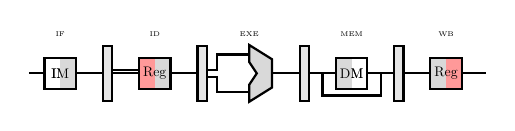
\begin{tikzpicture}[scale=0.5, transform shape]
            % Define styles
            \tikzstyle{block} = [rectangle, draw, thick, minimum width=0.8cm, minimum height=0.8cm, inner sep=2pt]
            \tikzstyle{latch} = [rectangle, draw, thick, minimum width=0.12cm, minimum height=1.4cm, fill=gray!20]
            \tikzstyle{line} = [draw, thick]
            
            % Stage labels
            \node[above] at (0,0.8) {\tiny IF};
            \node[above] at (2.4,0.8) {\tiny ID};
            \node[above] at (4.8,0.8) {\tiny EXE};
            \node[above] at (7.4,0.8) {\tiny MEM};
            \node[above] at (9.8,0.8) {\tiny WB};
            
            % Single pipeline row components
            \node[block, fill=white] (IM) at (0,0) {IM};
            \fill[gray!30] (IM.north) -- (IM.north east) -- (IM.south east) -- (IM.south) -- cycle;
            \node[block, fill=none] at (0,0) {IM};
            
            \node[latch] (L1) at (1.2,0) {};
            
            % Highlight Reg for READ (left half)
            \node[block, fill=white] (Reg1) at (2.4,0) {Reg};
            \fill[red!40] (Reg1.north west) -- (Reg1.north) -- (Reg1.south) -- (Reg1.south west) -- cycle;
            \fill[gray!30] (Reg1.north) -- (Reg1.north east) -- (Reg1.south east) -- (Reg1.south) -- cycle;
            \node[block, fill=none] at (2.4,0) {Reg};
            
            \node[latch] (L2) at (3.6,0) {};
            
            % ALU
            \begin{scope}[shift={(4.8,0)}, scale=1.2]
                \coordinate (toptopleft) at (0, 0.6);
                \coordinate (topbottomleft) at (0, 0.24);
                \coordinate (left) at (0.16, 0);
                \coordinate (bottomtopleft) at (0, -0.24);
                \coordinate (bottombottomleft) at (0, -0.6);
                \coordinate (topright) at (0.48, 0.3);
                \coordinate (bottomright) at (0.48, -0.3);
                \fill[gray!30] (toptopleft) -- (topbottomleft) -- (left) -- (bottomtopleft) -- (bottombottomleft) -- (bottomright) -- (topright) -- cycle;
                \draw[thick] (toptopleft) -- (topbottomleft) -- (left) -- (bottomtopleft) -- (bottombottomleft) -- (bottomright) -- (topright) -- cycle;
                \coordinate (alu_input1) at (0, 0.4);
                \coordinate (alu_input2) at (0, -0.4);
                \coordinate (alu_output) at (0.48, 0);
            \end{scope}
            
            \node[latch] (L3) at (6.2,0) {};
            
            \node[block, fill=white] (DM) at (7.4,0) {DM};
            \fill[gray!30] (DM.north west) -- (DM.north) -- (DM.south) -- (DM.south west) -- cycle;
            \node[block, fill=none] at (7.4,0) {DM};
            
            \node[latch] (L4) at (8.6,0) {};
            
            % Highlight Reg for WRITE (right half)
            \node[block, fill=white] (Reg2) at (9.8,0) {Reg};
            \fill[gray!30] (Reg2.north west) -- (Reg2.north) -- (Reg2.south) -- (Reg2.south west) -- cycle;
            \fill[red!40] (Reg2.north) -- (Reg2.north east) -- (Reg2.south east) -- (Reg2.south) -- cycle;
            \node[block, fill=none] at (9.8,0) {Reg};
            
            % Connections
            \draw[line] (-0.8,0) -- (IM.west);
            \draw[line] (IM.east) -- (L1.west);
            
            % Two inputs to first Reg (from different sources)
            \draw[line] ([yshift=2.4pt]L1.east) -- ([yshift=2.4pt]Reg1.west);
            \draw[line] (L1.east) -- (Reg1.west);
            
            \draw[line] (Reg1.east) -- (L2.west);
            
            % Two inputs to ALU
            \draw[line] ([yshift=2.4pt]L2.east) -- ++(0.24,0) |- (alu_input1);
            \draw[line] ([yshift=-2.4pt]L2.east) -- ++(0.24,0) |- (alu_input2);
            
            % ALU output to next latch
            \draw[line] (alu_output) -- (L3.west);
            
            % DM connections
            \draw[line] (L3.east) -- (DM.west);
            \draw[line] (DM.east) -- (L4.west);
            
            % Bypass around DM
            \draw[line] (L3.east) -- ($(L3.east)!0.5!(DM.west)$) -- ++(0, -0.56) -|
                        ($(L4.west)!0.5!(DM.east)$) -- (L4.west);
            
            \draw[line] (L4.east) -- (Reg2.west);
            \draw[line] (Reg2.east) -- ++(0.6,0);
        \end{tikzpicture}
        
        \column{0.45\textwidth}
        \textbf{Memory Contention:}
        \begin{itemize}
            \item Inst Fetch during IF (stage 1)
            \item Data access during MEM (stage 4)
            \item Solution: separate I\$ and D\$
        \end{itemize}
        
        \vspace{0.3cm}
        \centering
        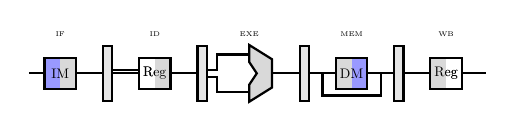
\begin{tikzpicture}[scale=0.5, transform shape]
            % Define styles
            \tikzstyle{block} = [rectangle, draw, thick, minimum width=0.8cm, minimum height=0.8cm, inner sep=2pt]
            \tikzstyle{latch} = [rectangle, draw, thick, minimum width=0.12cm, minimum height=1.4cm, fill=gray!20]
            \tikzstyle{line} = [draw, thick]
            
            % Stage labels
            \node[above] at (0,0.8) {\tiny IF};
            \node[above] at (2.4,0.8) {\tiny ID};
            \node[above] at (4.8,0.8) {\tiny EXE};
            \node[above] at (7.4,0.8) {\tiny MEM};
            \node[above] at (9.8,0.8) {\tiny WB};
            
            % Single pipeline row components
            % Highlight IM for instruction fetch (READ - left side)
            \node[block, fill=white] (IM) at (0,0) {IM};
            \fill[blue!40] (IM.north west) -- (IM.north) -- (IM.south) -- (IM.south west) -- cycle;
            \fill[gray!30] (IM.north) -- (IM.north east) -- (IM.south east) -- (IM.south) -- cycle;
            \node[block, fill=none] at (0,0) {IM};
            
            \node[latch] (L1) at (1.2,0) {};
            
            \node[block, fill=white] (Reg1) at (2.4,0) {Reg};
            \fill[gray!30] (Reg1.north) -- (Reg1.north east) -- (Reg1.south east) -- (Reg1.south) -- cycle;
            \node[block, fill=none] at (2.4,0) {Reg};
            
            \node[latch] (L2) at (3.6,0) {};
            
            % ALU
            \begin{scope}[shift={(4.8,0)}, scale=1.2]
                \coordinate (toptopleft) at (0, 0.6);
                \coordinate (topbottomleft) at (0, 0.24);
                \coordinate (left) at (0.16, 0);
                \coordinate (bottomtopleft) at (0, -0.24);
                \coordinate (bottombottomleft) at (0, -0.6);
                \coordinate (topright) at (0.48, 0.3);
                \coordinate (bottomright) at (0.48, -0.3);
                \fill[gray!30] (toptopleft) -- (topbottomleft) -- (left) -- (bottomtopleft) -- (bottombottomleft) -- (bottomright) -- (topright) -- cycle;
                \draw[thick] (toptopleft) -- (topbottomleft) -- (left) -- (bottomtopleft) -- (bottombottomleft) -- (bottomright) -- (topright) -- cycle;
                \coordinate (alu_input1) at (0, 0.4);
                \coordinate (alu_input2) at (0, -0.4);
                \coordinate (alu_output) at (0.48, 0);
            \end{scope}
            
            \node[latch] (L3) at (6.2,0) {};
            
            % Highlight DM for data access (READ/WRITE - right side)
            \node[block, fill=white] (DM) at (7.4,0) {DM};
            \fill[gray!30] (DM.north west) -- (DM.north) -- (DM.south) -- (DM.south west) -- cycle;
            \fill[blue!40] (DM.north) -- (DM.north east) -- (DM.south east) -- (DM.south) -- cycle;
            \node[block, fill=none] at (7.4,0) {DM};
            
            \node[latch] (L4) at (8.6,0) {};
            
            \node[block, fill=white] (Reg2) at (9.8,0) {Reg};
            \fill[gray!30] (Reg2.north west) -- (Reg2.north) -- (Reg2.south) -- (Reg2.south west) -- cycle;
            \node[block, fill=none] at (9.8,0) {Reg};
            
            % Connections
            \draw[line] (-0.8,0) -- (IM.west);
            \draw[line] (IM.east) -- (L1.west);
            
            % Two inputs to first Reg (from different sources)
            \draw[line] ([yshift=2.4pt]L1.east) -- ([yshift=2.4pt]Reg1.west);
            \draw[line] (L1.east) -- (Reg1.west);
            
            \draw[line] (Reg1.east) -- (L2.west);
            
            % Two inputs to ALU
            \draw[line] ([yshift=2.4pt]L2.east) -- ++(0.24,0) |- (alu_input1);
            \draw[line] ([yshift=-2.4pt]L2.east) -- ++(0.24,0) |- (alu_input2);
            
            % ALU output to next latch
            \draw[line] (alu_output) -- (L3.west);
            
            % DM connections
            \draw[line] (L3.east) -- (DM.west);
            \draw[line] (DM.east) -- (L4.west);
            
            % Bypass around DM
            \draw[line] (L3.east) -- ($(L3.east)!0.5!(DM.west)$) -- ++(0, -0.56) -|
                        ($(L4.west)!0.5!(DM.east)$) -- (L4.west);
            
            \draw[line] (L4.east) -- (Reg2.west);
            \draw[line] (Reg2.east) -- ++(0.6,0);
        \end{tikzpicture}
    \end{columns}
\end{frame}

\begin{frame}{Pipeline Architecture}
\begin{center}
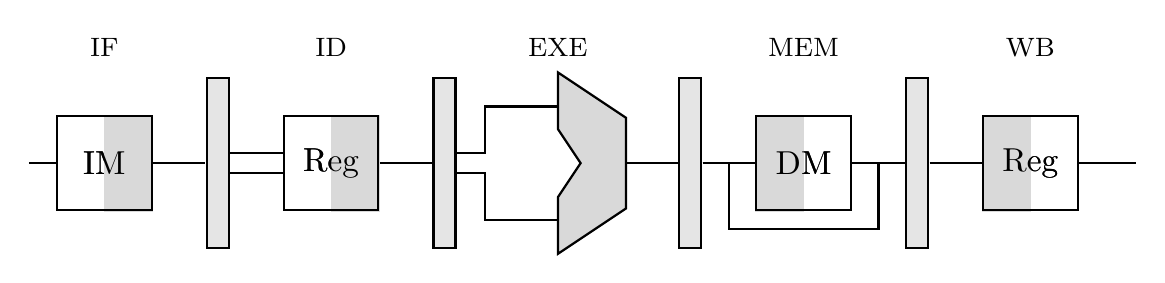
\begin{tikzpicture}[scale=1.2, transform shape]
    % Define styles
    \tikzstyle{block} = [rectangle, draw, thick, minimum width=1cm, minimum height=1cm, inner sep=2pt]
    \tikzstyle{latch} = [rectangle, draw, thick, minimum width=0.15cm, minimum height=1.8cm, fill=gray!20]
    \tikzstyle{line} = [draw, thick]
    
    % Stage labels
    \node[above, font=\footnotesize] at (0,1) {IF};
    \node[above, font=\footnotesize] at (2.4,1) {ID};
    \node[above, font=\footnotesize] at (4.8,1) {EXE};
    \node[above, font=\footnotesize] at (7.4,1) {MEM};
    \node[above, font=\footnotesize] at (9.8,1) {WB};
    
    % Single pipeline row components
    \node[block, fill=white] (IM) at (0,0) {IM};
    
    % Shade right half of IM (background)
    \fill[gray!30] (IM.north) -- (IM.north east) -- (IM.south east) -- (IM.south) -- cycle;
    % Redraw IM border and text on top
    \node[block, fill=none] at (0,0) {IM};
    
    % Latch after IM
    \node[latch] (L1) at (1.2,0) {};
    
    \node[block, fill=white] (Reg1) at (2.4,0) {Reg};
    
    % Shade right half of first Reg (background)
    \fill[gray!30] (Reg1.north) -- (Reg1.north east) -- (Reg1.south east) -- (Reg1.south) -- cycle;
    % Redraw Reg1 border and text on top
    \node[block, fill=none] at (2.4,0) {Reg};
    
    % Latch after Reg1
    \node[latch] (L2) at (3.6,0) {};
    
    % ALU using the custom shape (with gray shading)
    \begin{scope}[shift={(4.8,0)}, scale=1.2]
        % Trapezoid coordinates
        \coordinate (toptopleft) at (0, 0.8);
        \coordinate (topbottomleft) at (0, 0.3);
        \coordinate (left) at (0.2, 0);
        \coordinate (bottomtopleft) at (0, -0.3);
        \coordinate (bottombottomleft) at (0, -0.8);
        \coordinate (topright) at (0.6, 0.4);
        \coordinate (bottomright) at (0.6, -0.4);
        
        % Draw the trapezoid with gray fill
        \fill[gray!30] (toptopleft) -- (topbottomleft) -- (left) -- (bottomtopleft) -- (bottombottomleft) -- (bottomright) -- (topright) -- cycle;
        \draw[thick] (toptopleft) -- (topbottomleft) -- (left) -- (bottomtopleft) -- (bottombottomleft) -- (bottomright) -- (topright) -- cycle;
        
        % ALU connection points
        \coordinate (alu_input1) at (0, 0.5);
        \coordinate (alu_input2) at (0, -0.5);
        \coordinate (alu_output) at (0.6, 0);
    \end{scope}
    
    % Latch after ALU
    \node[latch] (L3) at (6.2,0) {};
    
    \node[block, fill=white] (DM) at (7.4,0) {DM};
    
    % Shade left half of DM for read, right half for write
    \fill[gray!30] (DM.north west) -- (DM.north) -- (DM.south) -- (DM.south west) -- cycle;
    % Redraw DM border and text on top
    \node[block, fill=none] at (7.4,0) {DM};
    
    % Latch after DM
    \node[latch] (L4) at (8.6,0) {};
    
    \node[block, fill=white] (Reg2) at (9.8,0) {Reg};
    
    % Shade left half of last Reg (background)
    \fill[gray!30] (Reg2.north west) -- (Reg2.north) -- (Reg2.south) -- (Reg2.south west) -- cycle;
    % Redraw Reg2 border and text on top
    \node[block, fill=none] at (9.8,0) {Reg};
    
    % Main horizontal connections
    \draw[line] (-0.8,0) -- (IM.west);
    \draw[line] (IM.east) -- (L1.west);
    
    % Two inputs to first Reg (from different sources)
    \draw[line] ([yshift=3pt]L1.east) -- ([yshift=3pt]Reg1.west);
    \draw[line] ([yshift=-3pt]L1.east) -- ([yshift=-3pt]Reg1.west);
    
    \draw[line] (Reg1.east) -- (L2.west);
    
    % Two inputs to ALU
    \draw[line] ([yshift=3pt]L2.east) -- ++(0.3,0) |- (alu_input1);
    \draw[line] ([yshift=-3pt]L2.east) -- ++(0.3,0) |- (alu_input2);
    
    % ALU output to next latch
    \draw[line] (alu_output) -- (L3.west);
    
    % DM connections
    \draw[line] (L3.east) -- (DM.west);
    \draw[line] (DM.east) -- (L4.west);
    
    % Bypass around DM (using relative positioning)
    \draw[line] (L3.east) -- ($(L3.east)!0.5!(DM.west)$) -- ++(0, -0.7) -|
                ($(L4.west)!0.5!(DM.east)$) -- (L4.west);
    
    % Single connection to final Reg
    \draw[line] (L4.east) -- (Reg2.west);
    
    \draw[line] (Reg2.east) -- ++(0.6,0);
    
\end{tikzpicture}
\end{center}
\end{frame}

%% Slide: Pipeline Example
\begin{frame}{Pipeline Example: cycle 1}
    \begin{columns}
        \column{0.4\textwidth}
        \begin{tabular}{ll}
            0 & \texttt{lw R10,9(R1)}\\
            4 & \texttt{sub R11,R2,R3}\\
            8 & \texttt{and R12,R4,R5}\\
            12 & \texttt{or R13,R6,R7}
        \end{tabular}
        
        \column{0.6\textwidth}
        \centering
        PC = 0
        \vspace{0.5cm}
        
        \begin{tikzpicture}[scale=0.6]
            \node[draw, dashed, minimum width=8cm, minimum height=3cm, align=center] {
                Pipeline State Diagram\\
                (Cycle 1)
            };
        \end{tikzpicture}
    \end{columns}
\end{frame}

%% Slide: RAW Dependency
\begin{frame}{RAW Dependency}
    \begin{columns}
        \column{0.5\textwidth}
        Program execution order:
        \begin{enumerate}
            \item \texttt{sub R2, R1, R3}
            \item \texttt{and R12, \textcolor{red}{R2}, R5}
            \item \texttt{or R13, R6, \textcolor{red}{R2}}
            \item \texttt{add R14, \textcolor{red}{R2}, \textcolor{red}{R2}}
            \item \texttt{sw R15, 100(\textcolor{red}{R2})}
        \end{enumerate}
        
        \column{0.5\textwidth}
        \centering
        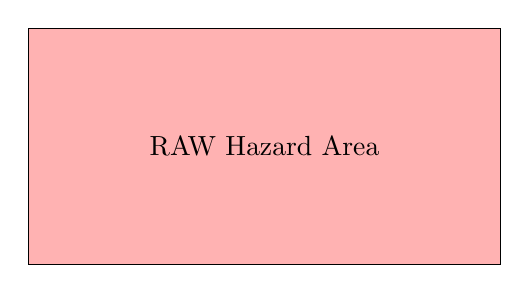
\begin{tikzpicture}[scale=0.5]
            % Pipeline stages showing dependency
            \node[draw, fill=red!30, minimum width=6cm, minimum height=3cm] {
                RAW Hazard Area
            };
        \end{tikzpicture}
    \end{columns}
\end{frame}

%% Slide: Using Bypass to Solve RAW Dependency
\begin{frame}{Using Bypass to Solve RAW Dependency}
    \begin{itemize}
        \item Bypass result directly from EXE output to EXE input
        \item No stall needed when bypass is possible
        \item Hardware forwards data from:
        \begin{itemize}
            \item EXE/MEM pipeline register
            \item MEM/WB pipeline register
        \end{itemize}
    \end{itemize}
    
    \centering
    \begin{tikzpicture}[scale=0.7]
        \node[draw, dashed, minimum width=10cm, minimum height=4cm] {
            Bypass/Forwarding Hardware Diagram
        };
    \end{tikzpicture}
\end{frame}

%% Slide: Bypass Control
\begin{frame}[fragile]{Bypass Control}
    \textbf{L3\_reg\_wr = L3.RegWrite and (L3.opcode != lw)}
    
    \vspace{0.3cm}
    \textbf{Forwarding from EXE (L3):}
    \begin{itemize}
        \item \small if (L3\_reg\_wr and (L3.dst == L2.src1)) ALUSelA = 1
        \item \small if (L3\_reg\_wr and (L3.dst == L2.src2)) ALUSelB = 1
    \end{itemize}
    
    \vspace{0.3cm}
    \textbf{Forwarding from MEM (L4):}
    \begin{itemize}
        \item \small if (L4.RegWrite and ((not L3\_reg\_wr) or (L3.dst $\neq$ L2.src1))\\
              and (L4.dst = L2.src1)) ALUSelA = 2
        \item \small if (L4.RegWrite and ((not L3\_reg\_wr) or (L3.dst $\neq$ L2.src2))\\
              and (L4.dst = L2.src2)) ALUSelB = 2
    \end{itemize}
\end{frame}

%% Slide: Register File Split
\begin{frame}{Register File Split}
    \begin{itemize}
        \item Register file is written during first half of the cycle
        \item Register file is read during second half of the cycle
        \item[$\Rightarrow$] Register file is written before it is read $\Rightarrow$ returns the correct data
    \end{itemize}
    
    \centering
    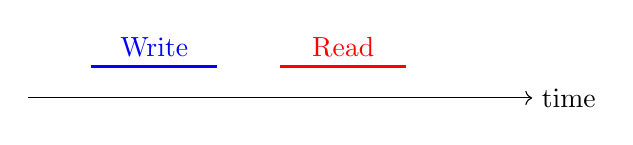
\begin{tikzpicture}[scale=0.8]
        % Timeline showing register file operations
        \draw[->] (0,0) -- (8,0) node[right] {time};
        \draw[thick, blue] (1,0.5) -- (3,0.5) node[midway, above] {Write};
        \draw[thick, red] (4,0.5) -- (6,0.5) node[midway, above] {Read};
    \end{tikzpicture}
\end{frame}

%% Slide: Can't Always Bypass
\begin{frame}{Can't Always Bypass}
    \begin{itemize}
        \item Load word can still cause a hazard
        \begin{itemize}
            \item An instruction tries to read a register following a load instruction that writes to the same register
        \end{itemize}
        \item A hazard detection unit is needed to "stall" the load instruction
    \end{itemize}
    
    Program execution order:
    \begin{enumerate}
        \item \texttt{lw \textcolor{red}{R2}, 30(R1)}
        \item \texttt{and R12, \textcolor{red}{R2}, R5}
        \item \texttt{or R13, R6, \textcolor{red}{R2}}
        \item \texttt{add R14, \textcolor{red}{R2}, \textcolor{red}{R2}}
        \item \texttt{sw R15, 100(\textcolor{red}{R2})}
    \end{enumerate}
\end{frame}

%% Slide: Stall If Cannot Bypass
\begin{frame}[fragile]{Stall If Cannot Bypass}
    \begin{verbatim}
if (L2.RegWrite and (L2.opcode == lw) and 
    ((L2.dst == L1.src1) or (L2.dst == L1.src2))) 
then stall
    \end{verbatim}
    
    \vspace{0.5cm}
    \begin{itemize}
        \item De-assert the enable to the L1 latch, and to the IP
        \begin{itemize}
            \item The dependent instruction (and) stays another cycle in L1
        \end{itemize}
        \item Issue a NOP into the L2 latch (instead of the stalled inst.)
        \item Allow the stalling instruction (lw) to move on
    \end{itemize}
    
    \centering
    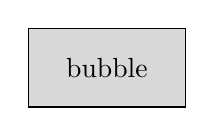
\begin{tikzpicture}[scale=0.6]
        \node[draw, fill=gray!30, minimum width=2cm, minimum height=1cm] {bubble};
    \end{tikzpicture}
\end{frame}

%% Slide: Software Scheduling to Avoid Load Hazards
\begin{frame}[fragile]{Software Scheduling to Avoid Load Hazards}
    Example: code for (assume all variables are in memory):
    \begin{center}
        \texttt{a = b + c;}\\
        \texttt{d = e - f;}
    \end{center}
    
    \begin{columns}
        \column{0.5\textwidth}
        \textbf{Slow code:}
        \begin{verbatim}
LW   Rb,b
LW   Rc,c
Stall
ADD  Ra,Rb,Rc
SW   a,Ra
LW   Re,e
LW   Rf,f
Stall
SUB  Rd,Re,Rf
SW   d,Rd
        \end{verbatim}
        
        \column{0.5\textwidth}
        \textbf{Fast code:}
        \begin{verbatim}
LW   Rb,b
LW   Rc,c
LW   Re,e
ADD  Ra,Rb,Rc
LW   Rf,f
SW   a,Ra
SUB  Rd,Re,Rf
SW   d,Rd
        \end{verbatim}
    \end{columns}
    
    \vspace{0.5cm}
    \centering
    \textit{Instruction order can be changed as long as the correctness is kept}
\end{frame}

\begin{frame}[label=control-hazard]{Control Hazard on Branches}
    \centering
    \drawPipelineDiagram[0,0.5]
    
    \vspace{0.5cm}
    \begin{center}
        \texttt{jcc target; if cond then PC $\leftarrow$ target}
        
        \vspace{0.2cm}
        \begin{minipage}{0.8\textwidth}
            \textcolor{green!70!black}{$\diamond$ The target is saved in the instruction relative to the address of the fall-through instruction}
            
            \textcolor{green!70!black}{$\diamond$ Most conditional jumps are short (if and loop) $\Rightarrow$ save bits in the instruction encoding}
        \end{minipage}
    \end{center}
\end{frame}

%% Slide: Control Hazard on Branches - With Annotations
\begin{frame}[label=control-hazard-annotated]{Control Hazard on Branches}
    \centering
    \drawPipelineDiagram[0,0.5]
    
    % Add annotations specific to this slide
    \begin{tikzpicture}[remember picture, overlay]
        % Add blue numbers for PC values
        \node[blue, font=\footnotesize\bfseries] at ($(current page.center) + (-6.4,-1.2)$) {8};
        \node[blue, font=\footnotesize\bfseries] at ($(current page.center) + (-3.7,1.4)$) {12};
        \node[blue, font=\footnotesize\bfseries] at ($(current page.center) + (-1.4,1.4)$) {8};
        \node[blue, font=\footnotesize\bfseries] at ($(current page.center) + (1.1,1.4)$) {4};
        
        % Add instruction labels in latches
        \node[font=\footnotesize\bfseries] at ($(current page.center) + (-3.05,-0.3)$) {jcc};
        \node[font=\footnotesize\bfseries] at ($(current page.center) + (-0.7,-0.3)$) {or};
        
        % Add orange highlight around certain paths
        \draw[orange!50, very thick, rounded corners] ($(current page.center) + (-7.0,0.9)$) rectangle ($(current page.center) + (6.4,3.1)$);
        
        % Add green highlight for decode stage
        \draw[green!50, very thick, rounded corners] ($(current page.center) + (-3.7,-1.5)$) rectangle ($(current page.center) + (-1.8,1.3)$);
        
        % Add text annotations at bottom
        \node[font=\footnotesize, align=left] at ($(current page.center) + (0,-3.0)$) {
            \texttt{jcc target; if cond then PC $\leftarrow$ target}
        };
        \node[font=\footnotesize, align=left, text=green!70!black] at ($(current page.center) + (0,-3.5)$) {
            $\diamond$ The target is saved in the instruction relative to the address of the fall-through instruction
        };
        \node[font=\footnotesize, align=left, text=green!70!black] at ($(current page.center) + (0,-4.0)$) {
            $\diamond$ Most conditional jumps are short (if and loop) $\Rightarrow$ save bits in the instruction encoding
        };
    \end{tikzpicture}
\end{frame}

%% Slide: Control Hazard: Stall
\begin{frame}{Control Hazard: Stall}
    \begin{itemize}
        \item Stall pipe when branch is encountered until resolved
        \item Stall impact: assumptions
        \begin{itemize}
            \item CPI = 1
            \item 20\% of instructions are branches
            \item Stall 3 cycles on every branch
            \item[$\Rightarrow$] $\text{CPI}_{\text{new}} = 1 + 0.2 \times 3 = 1.6$
        \end{itemize}
    \end{itemize}
    
    \vspace{0.5cm}
    \centering
    ($\text{CPI}_{\text{new}} = \text{CPI}_{\text{Ideal}} + \text{avg. stall cycles / instr.}$)
    
    \vspace{0.5cm}
    \textbf{We lose 60\% of the performance}
\end{frame}

%% Slide: Control Hazard: Stall  
\begin{frame}{Control Hazard: Stall}
    \begin{itemize}
        \item Stall pipe when branch is encountered until resolved
        \item Stall impact: assumptions
        \begin{itemize}
            \item CPI = 1
            \item 20\% of instructions are branches
            \item Stall 3 cycles on every branch
            \item[$\Rightarrow$] $\text{CPI}_{\text{new}} = 1 + 0.2 \times 3 = 1.6$
        \end{itemize}
    \end{itemize}
    
    \vspace{0.5cm}
    \centering
    ($\text{CPI}_{\text{new}} = \text{CPI}_{\text{Ideal}} + \text{avg. stall cycles / instr.}$)
    
    \vspace{0.5cm}
    \textbf{We lose 60\% of the performance}
\end{frame}

%% Slide: Control Hazard: Predict Not Taken
\begin{frame}{Control Hazard: Predict Not Taken}
    \begin{itemize}
        \item Execute instructions from the fall-through (not-taken) path
        \begin{itemize}
            \item As if there is no branch
            \item If the branch is not-taken ($\sim50\%$), no penalty is paid
        \end{itemize}
        \item If branch actually taken
        \begin{itemize}
            \item Flush the fall-through path instructions before they change the machine state (memory / registers)
            \item Fetch the instructions from the correct (taken) path
        \end{itemize}
        \item Assuming 20\% of instructions are branches and $\sim50\%$ branches not taken on average
        \begin{itemize}
            \item $\text{CPI}_{\text{new}} = 1 + (0.2 \times 0.5) \times 3 = 1.3$
        \end{itemize}
    \end{itemize}
\end{frame}

%% Slide: Dynamic Branch Prediction
\begin{frame}{Dynamic Branch Prediction}
    \begin{itemize}
        \item \textbf{Branch Target Buffer} (BTB) that predicts (at fetch)
        \begin{itemize}
            \item[$\diamond$] Instruction is a branch
            \item[$\diamond$] Branch taken / not-taken
            \item[$\diamond$] Taken branch target
        \end{itemize}
    \end{itemize}
    
    \vspace{0.3cm}
    
    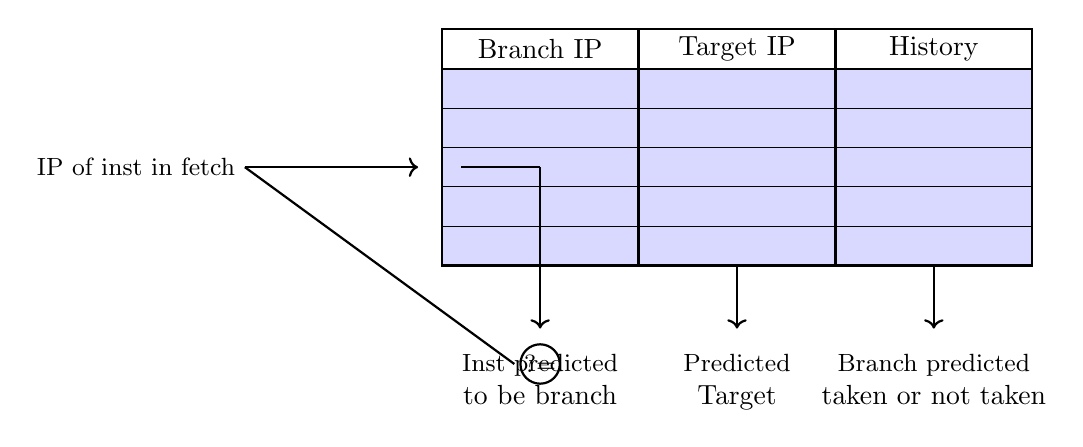
\begin{tikzpicture}[scale=1]
        % Draw the BTB table with light blue fill for data area
        \fill[blue!15] (0,0) rectangle (7.5,2.5);
        
        % Draw outer border
        \draw[thick] (0,0) rectangle (7.5,3);
        
        % Column dividers
        \draw[thick] (2.5,0) -- (2.5,3);
        \draw[thick] (5,0) -- (5,3);
        
        % Header row separator
        \draw[thick] (0,2.5) -- (7.5,2.5);
        
        % Data row lines (4 rows shown)
        \draw (0,2) -- (7.5,2);
        \draw (0,1.5) -- (7.5,1.5);
        \draw (0,1) -- (7.5,1);
        \draw (0,0.5) -- (7.5,0.5);
        
        % Header text
        \node at (1.25,2.75) {Branch IP};
        \node at (3.75,2.75) {Target IP};
        \node at (6.25,2.75) {History};
        
        % Arrow from "IP of inst in fetch" to comparison circle
        \draw[->,thick] (-2.5,1.25) -- (-0.3,1.25);
        \node[left] (ip) at (-2.5,1.25) {\small IP of inst in fetch};
        
        % Comparison circle positioned between arrow and Branch IP column
        \draw[thick,fill=white] (1.25,-1.25) circle (0.25);
        \node (qmark) at (1.25,-1.25) {\small ?=};
        \draw[thick] (ip.east) -- (qmark.west);
        
        % Connect comparison to Branch IP column (horizontal then down)
        \draw[thick] (0.25,1.25) -- (1.25,1.25);
        \draw[->,thick] (1.25,1.25) -- (1.25,0) -- (1.25,-0.8);
        
        % Arrow from Target IP column straight down
        \draw[->,thick] (3.75,0) -- (3.75,-0.8);
        
        % Arrow from History column straight down
        \draw[->,thick] (6.25,0) -- (6.25,-0.8);
        
        % Output labels
        \node[below,align=center] at (1.25,-1) {\small Inst predicted\\to be branch};
        \node[below,align=center] at (3.75,-1) {\small Predicted\\Target};
        \node[below,align=center] at (6.25,-1) {\small Branch predicted\\taken or not taken};
    \end{tikzpicture}
    
    \vspace{0.4cm}
    
    \begin{itemize}
        \item BTB allocated at execute -- after all branch info is known
        \item BTB is looked up at instruction fetch
    \end{itemize}
\end{frame}


%% Slide: BTB
\begin{frame}{BTB}
    \begin{itemize}
        \item \textbf{Allocation} - at Decode / EXE
        \begin{itemize}
            \item Allocate instructions identified as branches (after decode)
            \item Not taken branches need not be allocated
            \item BTB miss implicitly predicts not-taken
        \end{itemize}
        \item \textbf{Prediction} - at Fetch
        \begin{itemize}
            \item BTB lookup is done parallel to IC lookup
            \item BTB provides:
            \begin{itemize}
                \item Indication that the instruction is a branch (BTB hits)
                \item Branch predicted target
                \item Branch predicted direction
                \item Branch predicted type (e.g., conditional, unconditional)
            \end{itemize}
        \end{itemize}
        \item \textbf{Update} (when branch outcome is known - at EXE)
        \begin{itemize}
            \item Branch target
            \item Branch history (taken / not-taken)
        \end{itemize}
    \end{itemize}
\end{frame}

%% Slide: BTB (cont.)
\begin{frame}{BTB (cont.)}
    \begin{itemize}
        \item \textbf{Wrong prediction}
        \begin{itemize}
            \item Predict not-taken, actual taken
            \item Predict taken, actual not-taken, or actual taken but wrong target
        \end{itemize}
        \item \textbf{In case of wrong prediction – flush the pipeline}
        \begin{itemize}
            \item Reset latches (same as making all instructions to be NOPs)
            \item Select the PC source to be from the correct path
            \item Need get the fall-through with the branch
            \item Start fetching instruction from correct path
        \end{itemize}
        \item \textbf{Assuming P\% correct prediction rate}
        \begin{itemize}
            \item $\text{CPI}_{\text{new}} = 1 + (0.2 \times (1-P)) \times 3$
            \item For example, if P=0.7
            \item $\text{CPI}_{\text{new}} = 1 + (0.2 \times 0.3) \times 3 = 1.18$
        \end{itemize}
    \end{itemize}
\end{frame}

%% Slide: Adding a BTB to the Pipeline
\begin{frame}{Adding a BTB to the Pipeline}
    \centering
    \begin{tikzpicture}[scale=0.7]
        % Placeholder for BTB pipeline integration diagram
        \node[draw, rectangle, minimum width=14cm, minimum height=7cm, dashed, align=center] {
            \Large BTB Integration with Pipeline\\
            \normalsize BTB lookup parallel with I-cache lookup\\
            \small Predicted target and direction available at Fetch
        };
    \end{tikzpicture}
\end{frame}

%% Slide: Using The BTB
\begin{frame}{Using The BTB}
    \centering
    \tiny
    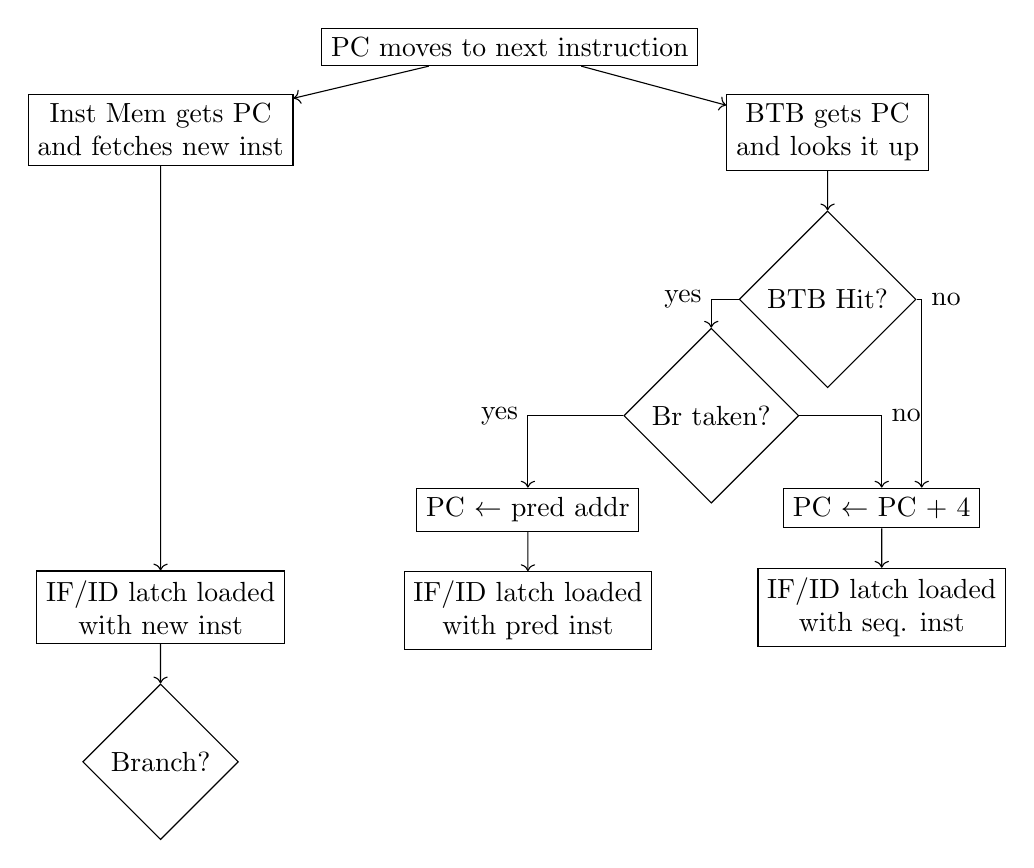
\begin{tikzpicture}[scale=0.8, node distance=0.5cm]
        % Flowchart for BTB usage
        \node[draw, rectangle] (pc) {PC moves to next instruction};
        \node[draw, rectangle, below left=of pc, align=center] (imem) {Inst Mem gets PC\\and fetches new inst};
        \node[draw, rectangle, below right=of pc, align=center] (btb) {BTB gets PC\\and looks it up};
        \node[draw, diamond, below=of btb] (hit) {BTB Hit?};
        \node[draw, diamond, below left=of hit] (taken) {Br taken?};
        \node[draw, rectangle, below left=of taken] (pred) {PC $\leftarrow$ pred addr};
        \node[draw, rectangle, below right=of taken] (inc) {PC $\leftarrow$ PC + 4};
        \node[draw, rectangle, below=of pred, align=center] (predinst) {IF/ID latch loaded\\with pred inst};
        \node[draw, rectangle, below=of inc, align=center] (seqinst) {IF/ID latch loaded\\with seq. inst};
        \node[draw, rectangle, align=center] (new) at (seqinst -| imem) {IF/ID latch loaded\\with new inst};
        \node[draw, diamond, below=of new, align=center] (branch) {Branch?};
        
        \draw[->] (pc) -- (imem);
        \draw[->] (pc) -- (btb);
        \draw[->] (btb) -- (hit);
        \draw[->] (hit) -| node[left] {yes} (taken);
        \draw[->] (hit) -| node[right] {no} ([xshift=6.5cm]inc);
        \draw[->] (taken.west) -| node[left] {yes} (pred);
        \draw[->] (taken) -| node[right] {no} (inc);
        \draw[->] (pred) -- (predinst);
        \draw[->] (inc) -- (seqinst);
        \draw[->] (imem) -- (new);
        \draw[->] (new) -- (branch);
    \end{tikzpicture}
\end{frame}

%% Slide: Using The BTB (cont.)
\begin{frame}{Using The BTB (cont.)}
    \centering
    \tiny
    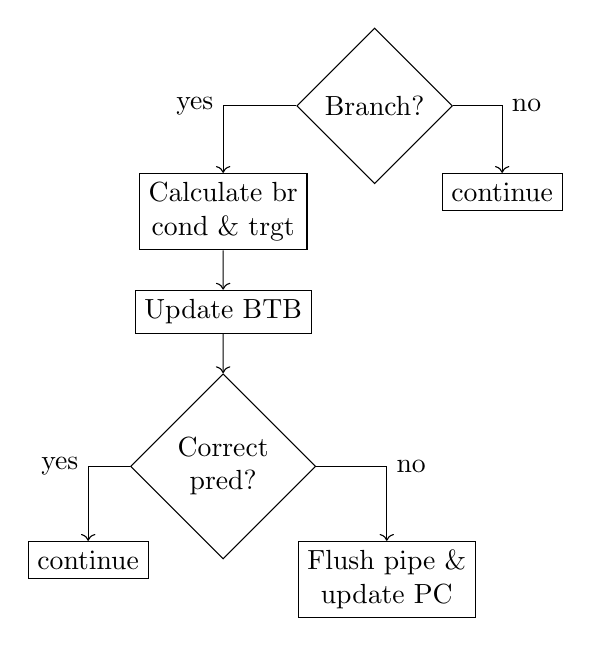
\begin{tikzpicture}[scale=0.8, node distance=0.5cm]
        % Continuation of BTB flowchart
        \node[draw, diamond] (branch) {Branch?};
        \node[draw, rectangle, below left=of branch, align=center] (calc) {Calculate br\\cond \& trgt};
        \node[draw, rectangle, below right=of branch] (continue1) {continue};
        \node[draw, rectangle, below=of calc] (update) {Update BTB};
        \node[draw, diamond, below=of update, align=center] (correct) {Correct\\pred?};
        \node[draw, rectangle, below right=of correct, align=center] (flush) {Flush pipe \&\\update PC};
        \node[draw, rectangle, below left=of correct] (continue2) {continue};
        
        \draw[->] (branch) -| node[left] {yes} (calc);
        \draw[->] (branch) -| node[right] {no} (continue1);
        \draw[->] (calc) -- (update);
        \draw[->] (update) -- (correct);
        \draw[->] (correct) -| node[right] {no} (flush);
        \draw[->] (correct) -| node[left] {yes} (continue2);
    \end{tikzpicture}
\end{frame}

\end{document}